%\onecolumn

\section{Experiments}
	\subsection{Finding the Wavelength}

\emph{NOTE: Do not send square waves or frequencies greater than 100Hz
to the Piezo, as this may result in damage.}

\begin{enumerate}
 	\item Set the function generator to a low frequency sinusoid.
		\begin{figure}[ht!]
		\centering
		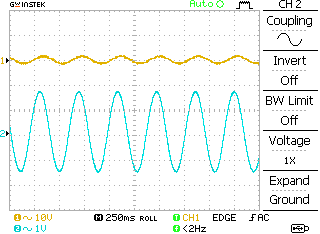
\includegraphics[width=2in]{DS0000}
		\end{figure}
	\item Connect the function generator's output to the oscilloscope's CH2
        and the Piezo via a T-connector.
	\item Using the scope, calculate the voltage difference required
		  to move the mirror through one complete fringe.
		\begin{figure}[ht!]
		\centering
		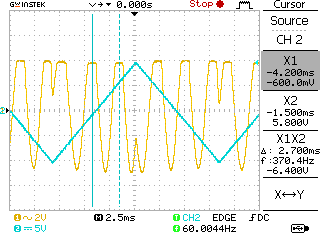
\includegraphics[width=2in]{DS0007}
		\end{figure}

	\emph{NOTE: Due to the mismatch in impedance (most function generators
		are 50 Ohm impedence), the amplitude seen by the piezo and scope is closer to 20 Vpp.}

\end{enumerate}



\textbf{Question 1:}
	
	\indent Using $\lambda_{experimental}$ calculate what $d$ must be
	if a group moves the test mirror and 1500 fringes pass through.

% measure voltages thru one complete fringe change. add picture. take multiple measurements, using run/stop command.

